\chapter{Introduction}\label{chp:introduction}

\epigraph{If I have seen further, it is by standing on the shoulders of giants}{Isaac Newton}

The web is becoming the primary platform for all communication. People are gradually moving away from solutions provided by their telco operator, such as telephony and text messaging, and over to Internet-based services. Moving audio conversations to the Internet has been relatively easy, but as we're now trying to commoditize video conversations, we have a bigger challenge ahead of us. Video conferencing has tradiationally been the domain of custom rooms and dedicated hardware, we're now trying to replicate that experience in regular laptops and phones. This has lead to performance requirements greater than most user equipment and their connections can handle. This thesis aims to lessen those performance requirements, and make video conferencing feasible in cases where it is not today.


\section{Problem}

Many new services for video conferencing have emerged in recent times, such as appear.in, Firefox Hello, and a host of others. Many of these are built on WebRTC, a standard for peer-to-peer communication in the browser. Without any further magic behind the scenes, such solutions will demand a linear increase in bandwidth both up and down as the number of peers in a conversation grows. This follows from the fact that in a peer-to-peer video conference, each peer has to encode it's own video to each of the other peers, send it to each of those peers, and receive that peer's video. This is expensive in terms of both CPU and bandwidth, and quickly outgrows what's actually available on many devices.

However, many other video conferencing solutions does not have this problem, as they ship all video through their own servers. Skype, Google Hangouts, custom rooms -- none of those has this scalability problem\footnote{They do however have another scalability problem: They number of servers they need to accomodate their users grows linearly with the total number of users on the platform.}. On the downside, they also don't have the small latency that can be achieved when you route video directly to the receiver, like you do in a peer-to-peer topology. They are also much costlier to operate, peer-to-peer systems only require a provider to help peers find each other, and will never see any of the actual video being transmitted\footnote{Generally. In some cases video will be transmitted through the provider for NAT-traversal, but bear with me.}. Which begs the question at the heart of this thesis -- can we design a solution that transcends these boundaries and provides high quality service for all combinations of user equipment and connections, without being expensive to run?

Formally put, we're looking to maximize the system's \emph{utility}. If you want to consider the full picture with users influenced by mood, context and lots of other human factors that come into play, this is a complex topic that could warrant several papers on its own. In this thesis we'll simplify the problem to only consider two factors that influence our decision: bandwidth and latency\footnote{I do however hope that the solution is general enough that we can expand it to include more factors eventually. CPU for example is another very constrained resource that preferably should be accounted for.}. Maximizing utility to us thus means delivering video between all parties in a conversation, at maximum bandwidth with minimal latency. This will be more formally specified in \autoref{chp:suggested-solution}. But what does utility really mean for a user?


\section{Utility}

Wiktionary \cite{wiki-utility} has a great definition of utility that can serve as a basis for this discussion.

\begin{description}
    \item[utility /\textipa{ju:" tIl.I.ti}/]  The ability of a commodity to satisfy needs or wants; the satisfaction experienced by the consumer of that commodity.
\end{description}

When a user evaluates the utility of a video conference service, context is everything. You have different expectations to audiovisual quality on a desktop computer with fiber connectivity compared to your phone on 3G. But how can this difference be quantized? Certainly it's not a question of screen resolution, as most smart phones today have the same 1080p resolution as most computer screens. Resolutions beyond 1080p, like we can find on some ``retina'' screens, are not that interesting for video conferencing, as the webcam producing the source video is unlikely to able to to the full potential of the screen.

However, physical screen size matters. Viewing distance matters. Latency matters very much. Bandwidth matters. Packet loss matters. Most of these should be fairly easy to estimate, but then we have a new problem: which of these attributes do we prioritize? Finding a balance here is key to a maximize service utility. There are of course also non-technical factors that affects the expected experience quite much that cannot be determined by the device itself. For example, you'll have different expectations sitting on the bus to work compared to sitting in a sofa in your living room, even though the device (and possibly also the connection) is the same. Content matters. Environment matters. Mood matters. Time of day probably matters. We will however not take all of these factors into account, but limit our scope to the device and the connection, and since the intended platform is WebRTC, what we can relatively easily determine through a web browser.

We assume that for each user, his experienced utility of the service will be a function of these variables that will follow the general shape of \autoref{fig:utility}. The important point here is the shape of the graph: there are diminishing returns. For smaller devices these will set in earlier, but they present for all devices. This ensures that we can specify a function that yields the utility for a user, and maximizing the outcome of this function will return fair results as to each device's potential.

\begin{figure}
    \centering
    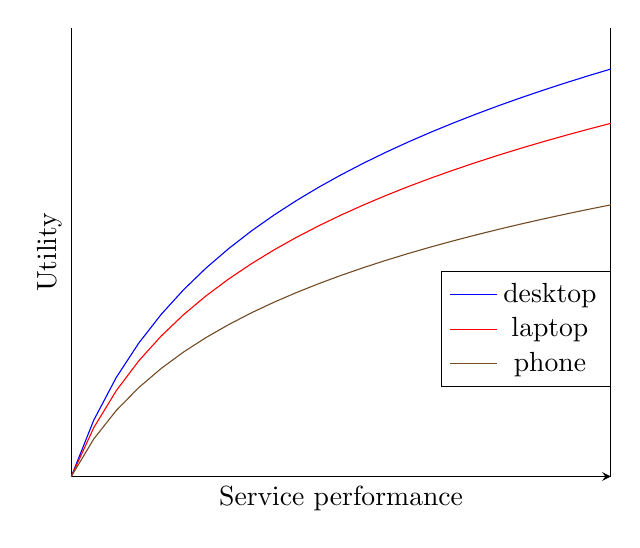
\begin{tikzpicture}
        \begin{axis}[
            xlabel=Service performance,
            ylabel=Utility,
            xmin=1,
            xmax=10,
            ymin=0,
            x axis line style={->},
            ticks=none,
            major x tick style = {opacity=1},
            minor tick length=0pt,
            axis x line=bottom,
            legend style={at={(1,0.20)}, anchor=south east,legend columns=1},
            ]

            \addplot+[domain=1:10,mark=none]{1.5*ln(x)};
            \addlegendentry{desktop}

            \addplot+[domain=1:10,mark=none]{1.3*ln(x)};
            \addlegendentry{laptop}

            \addplot+[domain=1:10,mark=none]{ln(x)};
            \addlegendentry{phone}

        \end{axis}
    \end{tikzpicture}
    \caption{Utility as a function of performance for different devices}
    \label{fig:utility}
\end{figure}


\section{Structure and Methodology}

Beforing trying to solve the problem we'll first evaluate the current video conferencing landscape in \autoref{chp:background}, to get a sense of the status quo. To limit the scope of what we're trying to accomplish, I'll define some test cases in \autoref{chp:test-cases} that we'll use throughout the thesis. We'll also evaluate one of the providers on the market today in \autoref{chp:experiments} by putting it to the test, running all the test cases from \autoref{chp:test-cases} to see how the service performs. Knowing this benchmark helps us evaluate the potential for my solution, which we'll take a look at in \autoref{chp:suggested-solution}. We'll discuss how our solution can be implemented and its strengths and weaknesses in \autoref{chp:discussion}, before summarizing what we've learned in \autoref{chp:conclusions}.


\section{Contribution}

This thesis proposes one way of modelling video conferences with known inter-node latencies and bandwidths as a flow network, and shows how an efficient routing for video can be derived from the model using linear programming. The method also demonstrates how performance can get a significant boost by adding extra nodes to the flow network acting as repeaters and transcoders, bridging the performance gap between traditional \gls{mcu}-backed solutions and peer-to-peer solutions.

I also benchmark the two most popular web browsers as of the time of writing, Google Chrome and Mozilla Firefox, in a set of test cases, and reveal severe flaws in how Firefox handles constrained nodes. Both browsers are shown to have lots of potential for increased performance. These tests were run with tools developed for this purpose, which are included in the appendices.


\section{Previous and Related Work}

Networking and algorithms related to networking is not a new topic, by any stretch of the imagination, and like in all most branches of computer science, it's mostly old problems in a new context.

During this thesis we will borrow heavily from previous work on networking and graph algorithms in general, and flow algorithms in particular. Many algorithmic problems can be solved as a linear program, which as a problem was first solved by Fourier in 1827 \cite{sierksma2001linear}. Another solution, the simplex method, was first introduced by G.B. Dantzig in 1947 \cite{sierksma2001linear}, and serves as the basis for the \gls{lp}-solver we'll use for our solution. The topic was introduced to me in \cite{ahuja1988network} by Ahuja, Magnanti and Orlin, which establishes the fundamentals for the flow-problem solution proposed later in this thesis. The simplex method has been widely adopted for its ease of implementation on computers, and years of exponential growth of computer performance has made solving increasingly large problem sets feasible.

A study at Chalmers in 2014 \cite{tree-topology-webrtc} investigated the feasibility of utilizing normal nodes in a video conference as supernodes, routing traffic from less powerful nodes through these nodes to reduce network load. The authors conclude that such a solution is feasible given proper supernode selection, which gives even greater possibilities for a solution utilizing dynamic topologies like presented in this thesis. Pushing as much traffic as possible over client-provided supernodes lowers the cost for the provider, and enables better quality for the users since peers can be closer to each other than to the closest data center. As the study concluded with supernodes being feasible and beneficial, my method is developed to be flexible enough to allow nodes to forward video to other nodes.

Now that we've established the problem domain and have some grasp of the main challenges, let's see where we are today.


\section{Notation and Terminology}

Bandwidth will often be written like this: 10/5. That should be read as 10Mbit download and 5Mbit upload, unless another unit is specified.

A video conference will often be called a conversation in this thesis. The term ``video conferencing'' carries a lot of luggage from its early history, when the technology was cumbersome, expensive, and only applicable in business scenarios. The movement WebRTC represents is about the opposite, commoditizing the technology to make it cheap and accessible to everyone, allowing it to enter the private domain. Friends don't ``confer'' between themselves; they converse. Names say a lot about a technology's intended application, thus if we want the technology to enter the private domain we need a name for it that does convey business usage. Hence the term used in this thesis: video conversations. The even less formal ``video chat'' could also have fit the bill, but that feels like it leaves the business side entirely in the dark; conversation feels like a good middle ground that is applicable to both sides.


\section{Disclaimer}

This thesis does not try to measure or solve for audio transmission, as that's a much simpler problem that can practically always be completed by sending the same stream to all nodes in the conversation. There's always only one stream to encode, it doesn't noticably affect available bandwidth, and it's already widely deployed. However, results we achieve for video can also be applied to audio streams if the environment is very heavily constrained or further optimization is required, but is out of scope for this thesis.
